\section{Implementierung}
\label{sec:implementation}
\subsection{List-based set with coarse-grained locks}

Bei dieser Implementierung wir vor jedem Methodenaufruf die gesamte Liste gesperrt. Dadurch kann aber die Parallelisierung 
nicht ausgenutzt werden, da zu einem Zeitpunkt maximal ein Prozess auf die Liste zugreifen kann. Diese Implementierung ist 
daher sehr ähnlich zu einer sequentiellen Implementierung.

\begin{figure}[H]
	\centering
    \begin{tikzpicture}
        \draw (-0.5,1) -- (10.5,1) node [midway, above, sloped] {\faLock};
		\node[draw,circle,minimum size=1cm,inner sep=0pt] at (0,0) {$- \infty$};
		\draw[->] (0.5,0) -- (1.5,0);
		\node[draw,circle,minimum size=1cm,inner sep=0pt] at (2,0) {$3$};
		\draw[->] (2.5,0) -- (3.5,0);
		\node[draw,circle,minimum size=1cm,inner sep=0pt] at (4,0) {$5$};
		\draw[->] (4.5,0) -- (5.5,0);
		\node[draw,circle,minimum size=1cm,inner sep=0pt] at (6,0) {$8$};
		\draw[->] (6.5,0) -- (7.5,0);
		\node[draw,circle,minimum size=1cm,inner sep=0pt] at (8,0) {$10$};
		\draw[->] (8.5,0) -- (9.5,0);
		\node[draw,circle,minimum size=1cm,inner sep=0pt] at (10,0) {$\infty$};
	\end{tikzpicture}
	\caption{coarse-grained locks}
	\label{tik:coarse-grained}
\end{figure}

\begin{table}[H]
    \begin{tabularx}{\textwidth}{lX}
        \textit{add} & Nachdem die Liste gesperrt wurde, wird sie durchlaufen bis zu dem Punkt, an dem der Key des betrachteten Nodes größer ist als der einzufügende ist. Vor diesen wird der neue Node eingefügt. \\
        \textit{contains} & Die Liste wird gesperrt und dann durchlaufen. Wenn dabei der gesuchten Wert gefunden wird, wird \textit{true}, ansonsten \textit{false} zurückgegeben.\\
        \textit{remove} & Nachdem die gesamte Liste gesperrt wurde wird das Element in der Liste gesucht und entfernt.\\
    \end{tabularx}
\end{table}

\subsection{List-based set with fine-grained locks}

Im Unterschied zu den \textit{coarse-grained locks} wird bei dieser Implementierung immer nur der derzeitige Node gesprerrt. 
Beim Iterieren der Liste wird während dem Übergang zum nächsten Node die derzeitige und der darauffolgende Node gesperrt. 
Ein Node kann zu einem Zeitpunkt nur von einem Prozess gesperrt sein. Der Vorteil gegenüber den coarse-grained locks besteht darin, 
dass nun wirkliche Parallelisierung möglich ist und verschiedene Threads an unterschiedlichen Punkten an der Liste arbeiten können. 
Es hat jedoch den Nachteil, dass die Iterationsgeschwiendigkeit durch den langsamsten Thread definiert wird, da ein 
Thread in der Liste nicht ``Überholt'' werden kann.

\begin{figure}[H]
	\centering
    \begin{tikzpicture}
        \draw (3.5,1) -- (4.5,1) node [midway, above, sloped] {\faLock};
        \draw (5.5,1) -- (6.5,1) node [midway, above, sloped] {\faLock};
		\node[draw,circle,minimum size=1cm,inner sep=0pt] at (0,0) {$- \infty$};
		\draw[->] (0.5,0) -- (1.5,0);
		\node[draw,circle,minimum size=1cm,inner sep=0pt] at (2,0) {$3$};
		\draw[->] (2.5,0) -- (3.5,0);
		\node[draw,circle,minimum size=1cm,inner sep=0pt] at (4,0) {$5$};
		\draw[->] (4.5,0) -- (5.5,0);
		\node[draw,circle,minimum size=1cm,inner sep=0pt] at (6,0) {$8$};
		\draw[->] (6.5,0) -- (7.5,0);
		\node[draw,circle,minimum size=1cm,inner sep=0pt] at (8,0) {$10$};
		\draw[->] (8.5,0) -- (9.5,0);
		\node[draw,circle,minimum size=1cm,inner sep=0pt] at (10,0) {$\infty$};
	\end{tikzpicture}
	\caption{fine-grained locks}
	\label{tik:fine-grained}
\end{figure}

\begin{figure}[H]
	\centering
    \begin{tikzpicture}
        \draw (3.5,1) -- (4.5,1) node [midway, above, sloped] {\faLock};
        \draw (5.5,-1) -- (6.5,-1) node [midway, above, sloped] {\faLock};
		\node[draw,circle,minimum size=1cm,inner sep=0pt] at (0,0) {$- \infty$};
		\draw[->] (0.5,0) -- (1.5,0);
		\node[draw,circle,minimum size=1cm,inner sep=0pt] at (2,0) {$3$};
		\draw[->] (2.5,0) -- (3.5,0);
		\node[draw,circle,minimum size=1cm,inner sep=0pt] at (4,0) {$5$};
        \draw[->] (4.5,0) -- (7.5,0);
        \draw[line width=0.5mm, red] (5.5,-1.5) -- (6.5,-2.5);
        \node[draw,circle,minimum size=1cm,inner sep=0pt] (A) at (6,-2) {$8$};
        \node[draw,circle,minimum size=1cm,inner sep=0pt] (B) at (8,0) {$10$};
        \draw[->] (A) -- (B);
		\draw[->] (8.5,0) -- (9.5,0);
		\node[draw,circle,minimum size=1cm,inner sep=0pt] at (10,0) {$\infty$};
	\end{tikzpicture}
	\caption{fine-grained locks remove}
	\label{tik:fine-grained-remove}
\end{figure}

\begin{table}[H]
    \begin{tabularx}{\textwidth}{lX}
		\textit{add} & Die Liste wird mit locks iteriert, bis der Punkt an dem der Node eingefügt werden soll erreich ist. Beim erreichen diese Punktes ist
		 sowohl der Vorgänger als auch der Nachfolger bereits gesperrt. Dadurch kann der neue Node sicher eingefügt werden.\\
		\textit{contains} & Die Liste wird analog zur coarse-grained locks iteriert, dabei aber immer der derzeitige Node bzw. beim Übergang Vorgänger und Nachfolger gesperrt. 
		Wenn der entsprechende Node gefunden wurde, wird \textit{true} sonst \textit{false} zurückgegeben. \\
		\textit{remove} & Die Liste wird wie bei \textit{contains} iteriert. Sobald der zu entfernende Node gefunden wurde, wird der Zeiger des vorgänger Nodes
		auf den darauffolgenden verwiesen und somit der zu entfernende Node übersprungen. Da der löschende Thread durch den lock exklusiven Zugriff auf den Node hat,
		kann dieser auch physikalisch vom Speicher entfernt werden. 
		Siehe Abbildung \ref{tik:fine-grained-remove}\\
    \end{tabularx}
\end{table}


\subsection{List-based set with optimistic synchronization}

In dieser Implementierung wird beim Suchen eines Elementes zuerst kein Node gesperrt, sondern einfach nur eine Iteration durchgeführt. 
Sobald der gesuchte gefunden wurde, wird dieser gesperrt. Anschließend muss sichergestellt werden, dass dieser Node noch immer erreichbar ist 
und nicht von einem anderen Thread bereits gelöscht wurde. Dies erfordert jedoch eine zweite Iteration der Liste. Ist der Node nicht mehr erreichbar, 
wird der Algorithmus von vorne gestartet. Dies hat den Vorteil, dass beim Suchen eines Keys in der Liste keine Sperrungen benötigt werden. 
Erst wenn das Element gefunden wurde, wird es gesperrt. Jedoch sind dadurch zwei Iterationen notwendig.

\begin{table}[H]
    \begin{tabularx}{\textwidth}{lX}
		\textit{add} & Beim Hinzufügen wird die Liste durchlaufen ohne Nodes zu sperren bis der entsprechende Punkt zum Einfügen gefunden wurde. 
		Die vorgänger und nachfolger Nodes werden gesperrt und mittels erneutem durchlaufen der Liste wird sichergestellt, dass diese Nodes immernoch Teil der 
		Liste sind. Falls dies scheitert wird der Prozess von vorne gestartet. Sind jedoch die gesperrten Nodes immernoch erreichbar, so wir der neue Key 
		zwischen den gesperrten eingefügt und die Sperre wird aufgehoben.\\
		\textit{contains} & Hier wird ebenfalls die Liste ohne Sperrungen durchsucht und nach Erfolgreichen Sperren plus der Validierung der Erreichbarkeit 
		der Nodes wird das Ergebnis zurückgegeben.\\
		\textit{remove} & Gleich wie bei den anderen Methoden wird der Key gesucht, gesperrt und validiert. Danach wird das Element aus der Liste entfernt und 
		alle Sperrungen werden aufgehoben. Da für das Iterieren keine Sperrungen erforderlich sind, kann nicht sichergestellt werden, dass der ausgelinkte
		Node nicht von einem anderen Thread gerade gelesen wird. Dadurch kann der Node nicht vom Speicher gelöscht werden.\\
    \end{tabularx}
\end{table}

Bei dieser Implementierung wurde auf Memory Managemen verzichtet, dadurch wird Speicher geleakt.
Eine Lösung dieses Problems wird in Kapitel \ref{sec:mem} gezeigt.

\subsection{List-based set with lazy synchronization}

Lazy Synchronization verwendet eine Markierung auf den Nodes welche bekannt gibt, ob dieser Node bereits logisch gelöscht wurde. 
Bei einem Lösch-Vorgang wird der zu löschenden Node diese Markierung gesetzt. Dadurch wird dieser Node bei anderen Methoden, 
wie zum Beispiel \textit{contain()} oder \textit{add()}, ignoriert. Dies hat den Vorteil, 
dass für den Aufruf von der \textit{contains()} Methode keine Sperrungen und keine Validierung erforderlich ist.
Dies bringt eine Performancesteigerung, da in der Regel mit \textit{contain()} die meisten Zugriffe auf die Datenstruktur erfolgen. 


\begin{figure}[H]
	\centering
    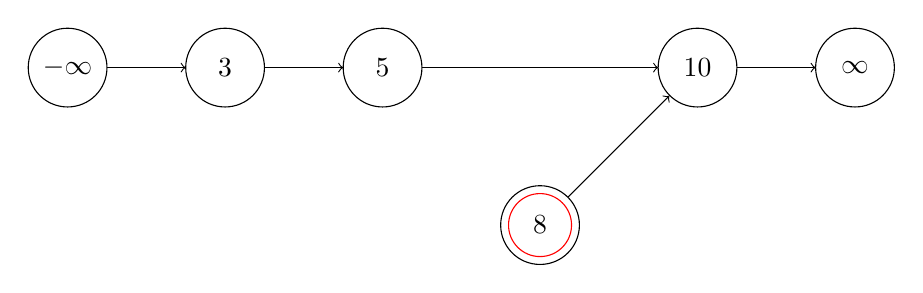
\begin{tikzpicture}
		\node[draw,circle,minimum size=1cm,inner sep=0pt] at (0,0) {$- \infty$};
		\draw[->] (0.5,0) -- (1.5,0);
		\node[draw,circle,minimum size=1cm,inner sep=0pt] at (2,0) {$3$};
		\draw[->] (2.5,0) -- (3.5,0);
		\node[draw,circle,minimum size=1cm,inner sep=0pt] at (4,0) {$5$};
        \draw[->] (4.5,0) -- (7.5,0);
        \node[draw,circle,minimum size=1cm,inner sep=0pt] (A) at (6,-2) {$8$};
        \node[draw,circle,minimum size=0.8cm,inner sep=0pt, red] at (6,-2) {};
        \node[draw,circle,minimum size=1cm,inner sep=0pt] (B) at (8,0) {$10$};
        \draw[->] (A) -- (B);
		\draw[->] (8.5,0) -- (9.5,0);
		\node[draw,circle,minimum size=1cm,inner sep=0pt] at (10,0) {$\infty$};
	\end{tikzpicture}
	\caption{fine-grained locks remove}
	\label{tik:fine-grained-remove}
\end{figure}

\begin{table}[H]
    \begin{tabularx}{\textwidth}{lX}
        \textit{add} & Gleich wie bei den optimistic synchronization\\
		\textit{contains} & Die Liste wird durchlaufen und bei einem erfolgreichem Fund wird sichergestellt, dass dieses Element noch nicht markiert wurde.
		Durch diese Markierung ist keine Validierung erforderlich. \\
		\textit{remove} & Der Key wird gesucht und mitsamt seinem Vorgänger gesperrt. Danach wird Validiert, ob dieses Element immernoch erreichbar ist. 
		Wenn dies der Fall ist wird das Element markiert und einseitig aus der Liste entfernt. Das bedeutet, dass dieser Node weiterhin auf den Nachfolger 
		zeigt, aber nicht mehr vom Kopf erreicht werden kann. Dies ist in Abbildung \ref{tik:fine-grained-remove} verdeutlicht. Dadurch kann wie bei
		optimistic synchronization der Node nicht vom Speicher entfernt werden.\\
    \end{tabularx}
\end{table}

Bei dieser Implementierung wurde auf Memory Managemen verzichtet, dadurch wird Speicher geleakt.
Eine Lösung dieses Problems wird in Kapitel \ref{sec:mem} gezeigt.



\subsection{Lock-free list-based set}

Das Ziel dieser Implementierung ist es eine sperrungsfreie Liste zu erstellen. Dazu wird ähnlich wie bei der \textit{lazy synchronization} eine Markierung verwendet. 
Diese Markierung wird aber in den next-Pointer des Nodes integriert, damit beide \textit{atomic} gelesen und geschrieben werden können. 
Um dies zu ermöglichen kann einfach ein Bit des Pointers genommen werden. Da bei einem 64-Bit Computer nicht alle Bits für die Adressierung 
des Speichers verwendet werden, kann das höchste Bit als Markierung umfunktioniert werden.

\begin{table}[H]
    \begin{tabularx}{\textwidth}{lX}
		\textit{add} & Bei add wird zuerst der Punkt zum Einfügen gesucht und dann wird ein neuer Node erzeugt, welcher auf den nachfolger Node zeigt. 
		Danach wird mittels \textit{compare\_exchange} der Vorgänger auf den neuen Node verwiesen und somit der neue Node in die Liste atomar eingefügt. 
		Scheitert \textit{compare\_exchange}, weil der next-Pointer vom Vorgänger von einem anderen Thread verändert wurde, wird der Prozess von Neuem gestartet. \\
        \textit{contains} & Gleich wie bei \textit{lazy synchronization} \\
		\textit{remove} & Bei remove wird der zu entfernende Node zuerst gesucht und dann im next-Pointer markiert. 
		Danach wird wieder mittels \textit{compare\_exchange} versucht 
		die Node noch aus der Liste zu entfernen indem in der Vorgänger Node der next-Pointer auf den Nachfolger gelegt wird. Falls dies jedoch scheitert werde 
		keine werteren Versuche zum Entfernen des Nodes aus der Liste vorgenommen. Die \textit{find()} Funktion, welche von \textit{add()}, \textit{contain()} und 
		\textit{remove()} verwendet wird, erkennt beim Iterieren markierte Nodes und versucht erneut diese zu entfernen. \\
    \end{tabularx}
\end{table}

\subsubsection{Verbesserungen}
\label{subsec:impr}
In der \textit{find} Funktion wird für das Auslinken eines Nodes wird ein Compare and Swap(CAS) verwendet. Falls dies fehlschlägt, 
weil z.b. der Node zum beispiel bereits ausgelinkt wurde,
wird wieder beim Listenkopf begonnen. Um dieses Verhalten zu verbessern, wurde in \textit{Lock\_free\_impr.cpp} folgendes implementiert:\\
Es wird immer der alte \textit{predecessor} gespeichert. Sollte CAS fehlschlagen, wird überprüft ob der alte \textit{predecessor}
zum auslinken markiert wurde. Ist dies der Fall, werden \textit{predecessor, current} und \textit{successor} auf den jeweiligen Vorgänger
gesetzt und an dieser Stelle weitergemacht. 